\documentclass[10pt]{beamer}
\usepackage{graphicx} % Required for inserting images
\usepackage{amssymb}
\usepackage{amsmath}
\usepackage{amsthm}
\usepackage{hyperref}
\usepackage{tikz} \usetikzlibrary{calc}
\usepackage{algpseudocode}
\usepackage{algorithm}
\usepackage{multirow}
\usepackage{tabularx}
\usepackage[table]{xcolor}
\usepackage{longtable}
\usepackage{subfigure}
\usepackage[most]{tcolorbox}
\usepackage{ulem}


\usetheme{Madrid}
\usecolortheme{seahorse}

\colorlet{myGray}{white!90!black}
\colorlet{myBlue}{blue!75!black}

\beamertemplatenavigationsymbolsempty
\setbeamertemplate{bibliography entry title}{}
\setbeamertemplate{bibliography entry location}{}
\setbeamertemplate{bibliography entry note}{}
\setbeamertemplate{bibliography item}{\insertbiblabel}
\setbeamercolor{bibliography item}{fg=black}
\setbeamercolor{bibliography entry author}{fg=black}
\setbeamercolor{bibliography entry title}{fg=black}
\setbeamercolor{bibliography entry location}{fg=black}
\setbeamercolor{bibliography entry note}{fg=black}
\setbeamertemplate{enumerate items}[default]

\newtcolorbox{mybox}{
    colback=white!95!black,
    frame hidden,
    enhanced jigsaw,
    breakable
    %fonttitle=\bfseries,
}

\newcommand{\code}[1]{\textcolor{myBlue}{\texttt{#1}}}

\title[PCCA]{\textbf{Modular integer arithmetic and SIMD vectorization using Intel AVX}}
\date{20 May 2025}
\author[D.ASSIRE, M.BONBOIRE]
{Damien ASSIRE \and Marie BONBOIRE}

\AtBeginSection[]
{
  \begin{frame}[noframenumbering]
    \frametitle{Table of Contents}
    \tableofcontents[currentsection, hideothersubsections]
  \end{frame}
}


\begin{document}

\begin{frame}[plain]
	\begin{center} 
		\includegraphics[scale=0.1]{su.png}
    \end{center}

    \titlepage
    
    \vfill
    \begin{flushleft}
        {\small
            \textbf{Supervisor:} Mr. Vincent NEIGER\footnote{\url{https://vincent.neiger.science/}} (LIP6 - PolSys)\\
        }
    \end{flushleft}
\end{frame}

\begin{frame}
    \frametitle{Table of Contents}
    \tableofcontents
\end{frame}

\section{Preface}
\begin{frame}
    \frametitle{Machines description}
    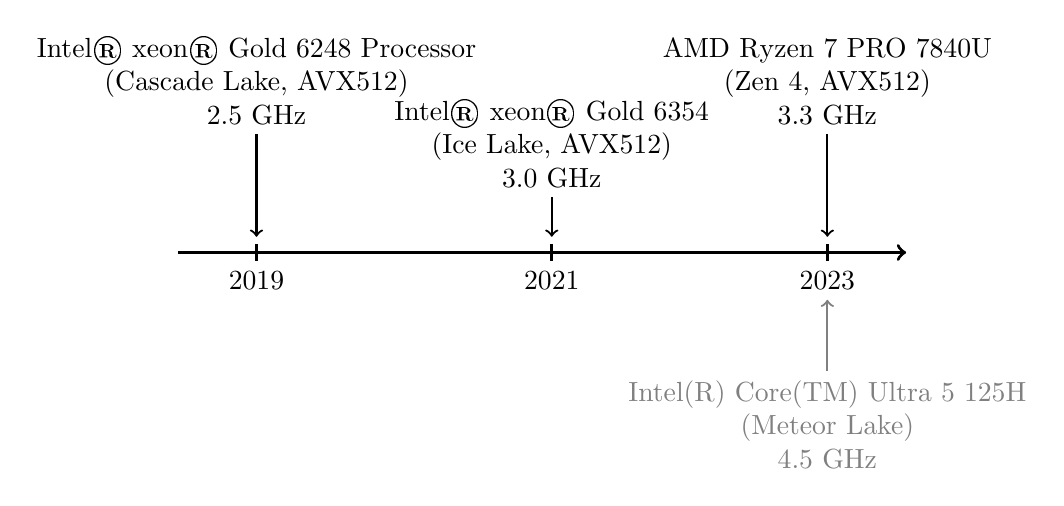
\begin{tikzpicture}[very thick, black]

        %coordinates
        \coordinate (O) at (0,0); % Origin
        \coordinate (F) at (9.25,0); %End
        \coordinate (P1) at (1,0); %ppti
        \coordinate (P2) at (4.75,0); %groebner
        \coordinate (P3) at (8.25,0); %mariz+argiope

        %proc
        \draw[<-,thick,color=black] ($(P1)+(0,0.2)$) -- ($(P1)+(0,1.5)$) node [above=0pt,align=center,black] 
        {Intel® xeon® Gold 6248 Processor \\ (Cascade Lake, AVX512) \\ 2.5 GHz};
        \draw[<-,thick,color=black] ($(P2)+(0,0.2)$) -- ($(P2)+(0,0.7)$) node [above=0pt,align=center,black] 
        {Intel® xeon® Gold 6354 \\ (Ice Lake, AVX512) \\ 3.0 GHz};
        \draw[<-,thick,color=black] ($(P3)+(0,0.2)$) -- ($(P3)+(0,1.5)$) node [above=0pt,align=center,black] 
        {AMD Ryzen 7 PRO 7840U \\ (Zen 4, AVX512) \\ 3.3 GHz};
        \draw[<-,thick,color=gray] ($(P3)-(0,0.6)$) -- ($(P3)-(0,1.5)$) node [below=0pt,align=center,gray] 
        {Intel(R) Core(TM) Ultra 5 125H \\ (Meteor Lake) \\ 4.5 GHz};

        %main arrow
        \draw[->] (O) -- (F);

        %ticks
        \foreach \x in {1,4.75,8.25}
        \draw(\x cm,3pt) -- (\x cm,-3pt);
        %labels
        \foreach \i \j in {1/2019,4.75/2021,8.25/2023}{
        	\draw (\i,0) node[below=3pt] {\j} ;
        }

\end{tikzpicture}
\end{frame}

\begin{frame}
    \begin{itemize}
        \item Vectorization
        \item Timings measurements
    \end{itemize}
\end{frame}

\section{Multiplication of 64-bit integers}
\subsection{Long multiplication}
\begin{frame}
    Long multiplication
\end{frame}

\subsection{Retrieve high and low part of the result}
\begin{frame}
    Low/high part of the result
\end{frame}

\subsection{Modular multiplication with a precomputation step}
\begin{frame}
    \frametitle{Modular multiplication with a precomputation step}

    \begin{example}
    Let $B$ be the maximum bitsize of a word ($B\in \{32, 64\}$). \\
    Given $n$ and $w \in \mathbb{Z}/n\mathbb{Z}$, one can compute a scaled approximation 
    of $\frac{w}{n}$, which is precisely $$ w_{pre} = \biggl\lfloor\dfrac{w\cdot 2^{B}}{n} \biggr\rfloor.$$
    \end{example}

    \bigskip
    For a vector $b = (b_1,\dots, b_N)$, one can compute 
    $$(w\cdot b_i \mod n) \text{ for each } i\in \{1, \dots, N\}$$

    using Shoup algorithm:

    \begin{enumerate}
        \item compute $p_{hi}, p_{lo}$ such that $w_{pre} \cdot b_i = p_{hi}\cdot 2^B + p_{lo}$, \hfill (1 \texttt{mulhi})
        \item compute $c = w\cdot b_i - p_{hi}\cdot n$, \hfill (2 \texttt{mullo})
        \item if $c \geq n$, return $c-n$, else return $c$ \\
            $\Longleftrightarrow \min(c-n, c)$.
    \end{enumerate}
\end{frame}

\section{Classic arithmetic operations on vectors}
\subsection{Addition of two vectors}
\begin{frame}
    Addition
\end{frame}

\subsection{Multiplication of a vector by a scalar}
\begin{frame}
    Scalar-vector
\end{frame}

\subsection{Dot product}
\begin{frame}
    1 - 2 slides
    dot product
\end{frame}

\section{Butterfly Fast Fourier Transform}
\subsection{Harvey lazy butterfly FFT}
\begin{frame}
    \frametitle{Harvey lazy butterfly FFT}
    \[
    (x,y) \mapsto (x + w\cdot y \mod n,\ x - w\cdot y \mod n).
    \]


\end{frame}

\subsection{Consequences on a complete FFT implementation}
\begin{frame}
    timings complete FFT
\end{frame}

\section{Conclusion}
\begin{frame}
    \begin{itemize}
        \item special primes
        \item ifma
    \end{itemize}
\end{frame}

\end{document}